\documentclass[american,]{article}
\usepackage{lmodern}
\usepackage{amssymb,amsmath}
\usepackage{ifxetex,ifluatex}
\usepackage{fixltx2e} % provides \textsubscript
\ifnum 0\ifxetex 1\fi\ifluatex 1\fi=0 % if pdftex
  \usepackage[T1]{fontenc}
  \usepackage[utf8]{inputenc}
\else % if luatex or xelatex
  \ifxetex
    \usepackage{mathspec}
  \else
    \usepackage{fontspec}
  \fi
  \defaultfontfeatures{Ligatures=TeX,Scale=MatchLowercase}
\fi
% use upquote if available, for straight quotes in verbatim environments
\IfFileExists{upquote.sty}{\usepackage{upquote}}{}
% use microtype if available
\IfFileExists{microtype.sty}{%
\usepackage{microtype}
\UseMicrotypeSet[protrusion]{basicmath} % disable protrusion for tt fonts
}{}
\usepackage[margin=1in]{geometry}
\usepackage{hyperref}
\hypersetup{unicode=true,
            pdftitle={Regression Analysis of Bike Sharing Demand},
            pdfauthor={Chance Robinson, Jayson Barker and Neha Dixit},
            pdfborder={0 0 0},
            breaklinks=true}
\urlstyle{same}  % don't use monospace font for urls
\ifnum 0\ifxetex 1\fi\ifluatex 1\fi=0 % if pdftex
  \usepackage[shorthands=off,main=american]{babel}
\else
  \usepackage{polyglossia}
  \setmainlanguage[variant=american]{english}
\fi
\usepackage{natbib}
\bibliographystyle{apalike}
\usepackage{color}
\usepackage{fancyvrb}
\newcommand{\VerbBar}{|}
\newcommand{\VERB}{\Verb[commandchars=\\\{\}]}
\DefineVerbatimEnvironment{Highlighting}{Verbatim}{commandchars=\\\{\}}
% Add ',fontsize=\small' for more characters per line
\usepackage{framed}
\definecolor{shadecolor}{RGB}{248,248,248}
\newenvironment{Shaded}{\begin{snugshade}}{\end{snugshade}}
\newcommand{\AlertTok}[1]{\textcolor[rgb]{0.94,0.16,0.16}{#1}}
\newcommand{\AnnotationTok}[1]{\textcolor[rgb]{0.56,0.35,0.01}{\textbf{\textit{#1}}}}
\newcommand{\AttributeTok}[1]{\textcolor[rgb]{0.77,0.63,0.00}{#1}}
\newcommand{\BaseNTok}[1]{\textcolor[rgb]{0.00,0.00,0.81}{#1}}
\newcommand{\BuiltInTok}[1]{#1}
\newcommand{\CharTok}[1]{\textcolor[rgb]{0.31,0.60,0.02}{#1}}
\newcommand{\CommentTok}[1]{\textcolor[rgb]{0.56,0.35,0.01}{\textit{#1}}}
\newcommand{\CommentVarTok}[1]{\textcolor[rgb]{0.56,0.35,0.01}{\textbf{\textit{#1}}}}
\newcommand{\ConstantTok}[1]{\textcolor[rgb]{0.00,0.00,0.00}{#1}}
\newcommand{\ControlFlowTok}[1]{\textcolor[rgb]{0.13,0.29,0.53}{\textbf{#1}}}
\newcommand{\DataTypeTok}[1]{\textcolor[rgb]{0.13,0.29,0.53}{#1}}
\newcommand{\DecValTok}[1]{\textcolor[rgb]{0.00,0.00,0.81}{#1}}
\newcommand{\DocumentationTok}[1]{\textcolor[rgb]{0.56,0.35,0.01}{\textbf{\textit{#1}}}}
\newcommand{\ErrorTok}[1]{\textcolor[rgb]{0.64,0.00,0.00}{\textbf{#1}}}
\newcommand{\ExtensionTok}[1]{#1}
\newcommand{\FloatTok}[1]{\textcolor[rgb]{0.00,0.00,0.81}{#1}}
\newcommand{\FunctionTok}[1]{\textcolor[rgb]{0.00,0.00,0.00}{#1}}
\newcommand{\ImportTok}[1]{#1}
\newcommand{\InformationTok}[1]{\textcolor[rgb]{0.56,0.35,0.01}{\textbf{\textit{#1}}}}
\newcommand{\KeywordTok}[1]{\textcolor[rgb]{0.13,0.29,0.53}{\textbf{#1}}}
\newcommand{\NormalTok}[1]{#1}
\newcommand{\OperatorTok}[1]{\textcolor[rgb]{0.81,0.36,0.00}{\textbf{#1}}}
\newcommand{\OtherTok}[1]{\textcolor[rgb]{0.56,0.35,0.01}{#1}}
\newcommand{\PreprocessorTok}[1]{\textcolor[rgb]{0.56,0.35,0.01}{\textit{#1}}}
\newcommand{\RegionMarkerTok}[1]{#1}
\newcommand{\SpecialCharTok}[1]{\textcolor[rgb]{0.00,0.00,0.00}{#1}}
\newcommand{\SpecialStringTok}[1]{\textcolor[rgb]{0.31,0.60,0.02}{#1}}
\newcommand{\StringTok}[1]{\textcolor[rgb]{0.31,0.60,0.02}{#1}}
\newcommand{\VariableTok}[1]{\textcolor[rgb]{0.00,0.00,0.00}{#1}}
\newcommand{\VerbatimStringTok}[1]{\textcolor[rgb]{0.31,0.60,0.02}{#1}}
\newcommand{\WarningTok}[1]{\textcolor[rgb]{0.56,0.35,0.01}{\textbf{\textit{#1}}}}
\usepackage{longtable,booktabs}
\usepackage{graphicx,grffile}
\makeatletter
\def\maxwidth{\ifdim\Gin@nat@width>\linewidth\linewidth\else\Gin@nat@width\fi}
\def\maxheight{\ifdim\Gin@nat@height>\textheight\textheight\else\Gin@nat@height\fi}
\makeatother
% Scale images if necessary, so that they will not overflow the page
% margins by default, and it is still possible to overwrite the defaults
% using explicit options in \includegraphics[width, height, ...]{}
\setkeys{Gin}{width=\maxwidth,height=\maxheight,keepaspectratio}
\IfFileExists{parskip.sty}{%
\usepackage{parskip}
}{% else
\setlength{\parindent}{0pt}
\setlength{\parskip}{6pt plus 2pt minus 1pt}
}
\setlength{\emergencystretch}{3em}  % prevent overfull lines
\providecommand{\tightlist}{%
  \setlength{\itemsep}{0pt}\setlength{\parskip}{0pt}}
\setcounter{secnumdepth}{5}
% Redefines (sub)paragraphs to behave more like sections
\ifx\paragraph\undefined\else
\let\oldparagraph\paragraph
\renewcommand{\paragraph}[1]{\oldparagraph{#1}\mbox{}}
\fi
\ifx\subparagraph\undefined\else
\let\oldsubparagraph\subparagraph
\renewcommand{\subparagraph}[1]{\oldsubparagraph{#1}\mbox{}}
\fi

%%% Use protect on footnotes to avoid problems with footnotes in titles
\let\rmarkdownfootnote\footnote%
\def\footnote{\protect\rmarkdownfootnote}

%%% Change title format to be more compact
\usepackage{titling}

% Create subtitle command for use in maketitle
\providecommand{\subtitle}[1]{
  \posttitle{
    \begin{center}\large#1\end{center}
    }
}

\setlength{\droptitle}{-2em}

  \title{Regression Analysis of Bike Sharing Demand}
    \pretitle{\vspace{\droptitle}\centering\huge}
  \posttitle{\par}
    \author{Chance Robinson, Jayson Barker and Neha Dixit}
    \preauthor{\centering\large\emph}
  \postauthor{\par}
      \predate{\centering\large\emph}
  \postdate{\par}
    \date{Master of Science in Data Science, Southern Methodist University, USA}

\usepackage{booktabs}
\usepackage{longtable}
\usepackage{array}
\usepackage{multirow}
\usepackage{wrapfig}
\usepackage{float}
\usepackage{colortbl}
\usepackage{pdflscape}
\usepackage{tabu}
\usepackage{threeparttable}
\usepackage{threeparttablex}
\usepackage[normalem]{ulem}
\usepackage{makecell}
\usepackage{xcolor}

\usepackage{amsmath}
\usepackage[utf8]{inputenc}
\usepackage[T1]{fontenc}
\usepackage{setspace}
\usepackage{hyperref}
\onehalfspacing
\setcitestyle{numbers,square,super}
\newcommand\numberthis{\addtocounter{equation}{1}\tag{\theequation}}

\begin{document}
\maketitle

\hypertarget{introduction}{%
\section{Introduction}\label{introduction}}

A bike sharing system is a means of renting a bicycle via a network of kiosk locations throughout a city and returning it to a different place as needed.

For this analysis, we are looking at two years' worth of bikeshare data from Capital Bikeshare in Washington D.C. Our data was retrieved from the \href{https://www.kaggle.com/c/bike-sharing-demand/overview}{\textit{
Bike Sharing Demand}} \cite{Kaggle2014} Kaggle competition.

The objective is to predict the total count of bikes rented during each hour covered by the test set.

\hypertarget{data-description}{%
\section{Data Description}\label{data-description}}

The dataset we chose for this project was a publicly shared, hourly bike sharing dataset made available through Kaggle in csv format.

This data set is divided into two distinct sets -- a train and test set. The train set consists of 10,886 rows (titled ``train.csv'') and the test set consists of 6,493 rows (titled ``test.csv''). Within the training set, the first 19 days of each month are captured whereas in the test data set, the 20th day to the end of each month is present. The entirety of the data spans from 1/1/2011 through 12/31/2012 - encompassing two full years of bike sharing data. Interestingly, the time component of this analysis is captured in hours of each day meaning we have a calendar date represented 24 times (for each hour of that day) in the data, along with it's associated attribute values.

\newpage

In train data set, there are a total of 12 attributes which capture multiple variables related to bike rentals. Some of these attributes are categorical, and others are continuous. All attributes are summarized in the table below:

\begin{longtable}[]{@{}lll@{}}
\toprule
Column Name & Type & Description\tabularnewline
\midrule
\endhead
1. datetime & Date & YYYY-MM-DD HH24 (example: 2011-01-01 04:00:00)\tabularnewline
2. season & Integer & (1-4)\tabularnewline
3. holiday & Integer & (0 or 1)\tabularnewline
4. workingday & Integer & (0 or 1)\tabularnewline
5. weather & Integer & (1-4)\tabularnewline
6. temp & Float & temparture in Celcius\tabularnewline
7. atemp & Float & ``feels like'' temperature in Celsius\tabularnewline
8. humidity & Integer & relative humidity\tabularnewline
9. windspeed & Float & wind speed\tabularnewline
10. casual & Integer & count of casual users\tabularnewline
11. registered & Integer & count of registered users\tabularnewline
12. count & Integer & count of total users (\emph{response variable})\tabularnewline
\bottomrule
\end{longtable}

\emph{Note that the test data set lacks the casual, registered and count variables.}

\newpage

\hypertarget{exploratory-data-analysis}{%
\section{Exploratory Data Analysis}\label{exploratory-data-analysis}}

\hypertarget{categorical-variables-plots}{%
\subsection{Categorical Variables Plots}\label{categorical-variables-plots}}

Several numeric variables were found to be better suited to categorization and were converted to factors.

\hypertarget{season}{%
\subsubsection{Season}\label{season}}

The Summer and Fall months show the highest seasonal averages.

\begin{longtable}[]{@{}lll@{}}
\toprule
Season & Label & Description\tabularnewline
\midrule
\endhead
1 & Spring & Dec 21 \textasciitilde{} Mar 20\tabularnewline
2 & Summer & Mar 21 \textasciitilde{} Jun 20\tabularnewline
3 & Fall & Jun 21 \textasciitilde{} Sep 20\tabularnewline
4 & Winter & Sep 21 \textasciitilde{} Dec 20\tabularnewline
\bottomrule
\end{longtable}

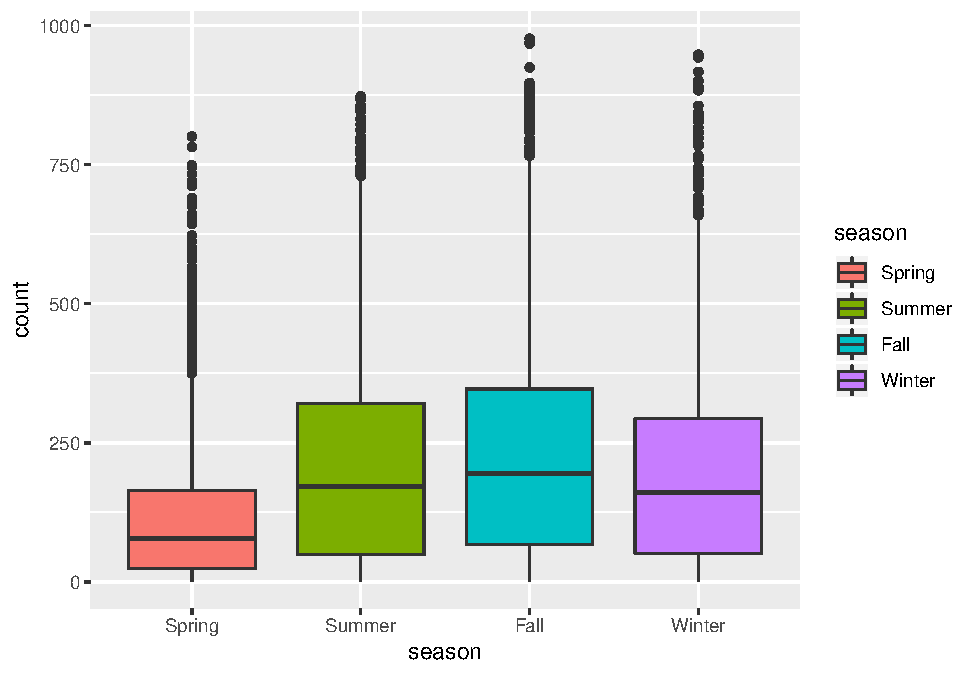
\includegraphics{BikeSharingDemand_files/figure-latex/train.mod.1.season-1.pdf}

\newpage

\hypertarget{holiday}{%
\subsubsection{Holiday}\label{holiday}}

Whether or not the day is a holiday, oddly enough, has no noticeable impact on the average counts.

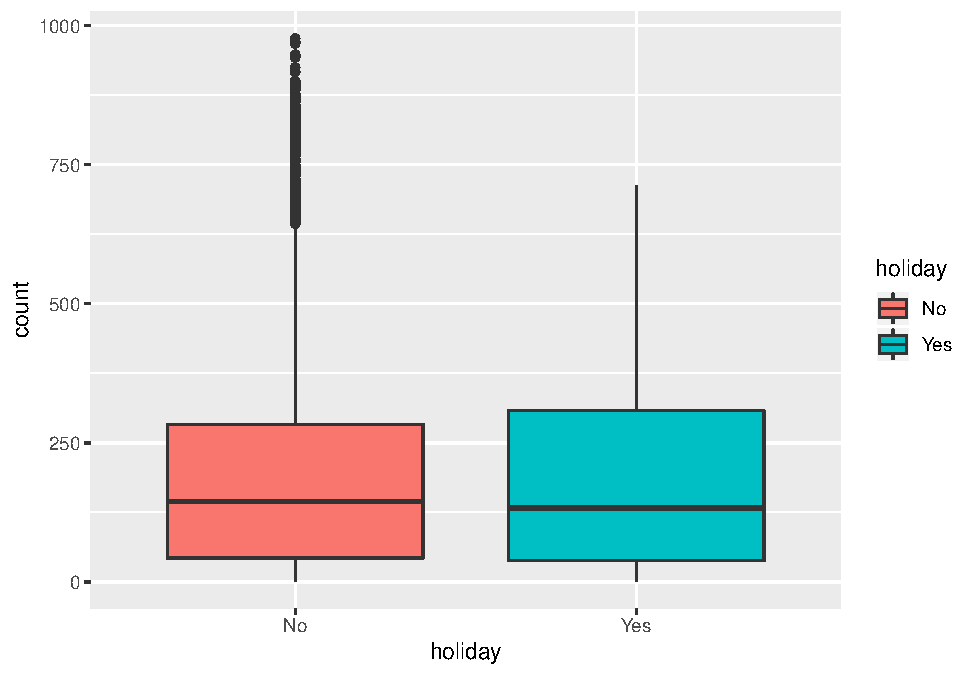
\includegraphics{BikeSharingDemand_files/figure-latex/train.mod.1.holiday-1.pdf}

\newpage

\hypertarget{working-day}{%
\subsubsection{Working Day}\label{working-day}}

The same could be said of whether or not the recording was on a working day or weekend.

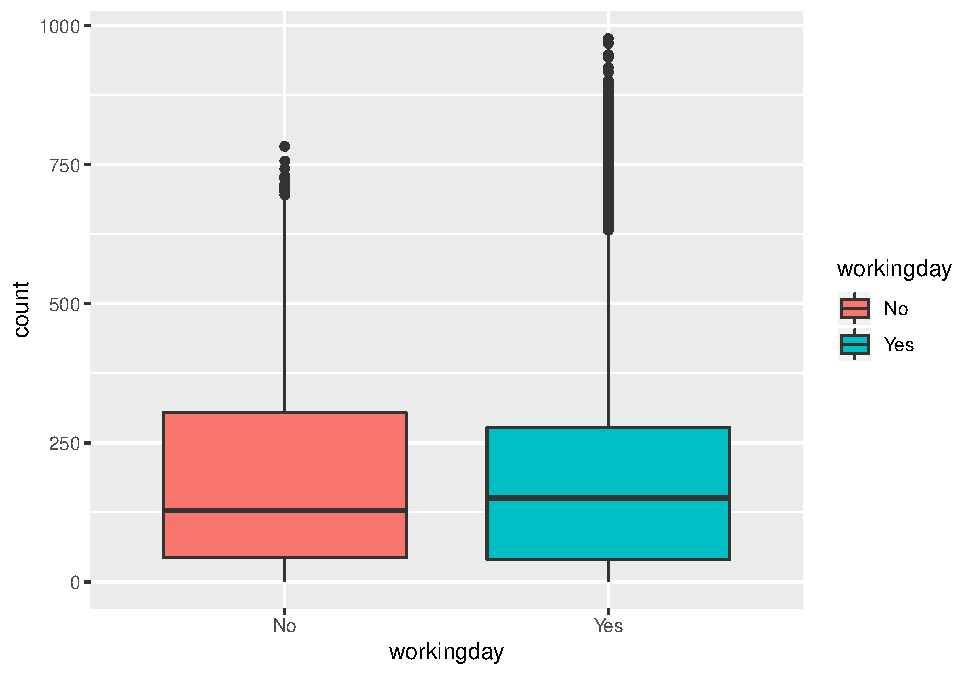
\includegraphics{BikeSharingDemand_files/figure-latex/train.mod.1.workingday-1.pdf}

\newpage

\hypertarget{weather}{%
\subsubsection{Weather}\label{weather}}

Better weather shows improved rental rates as expected.

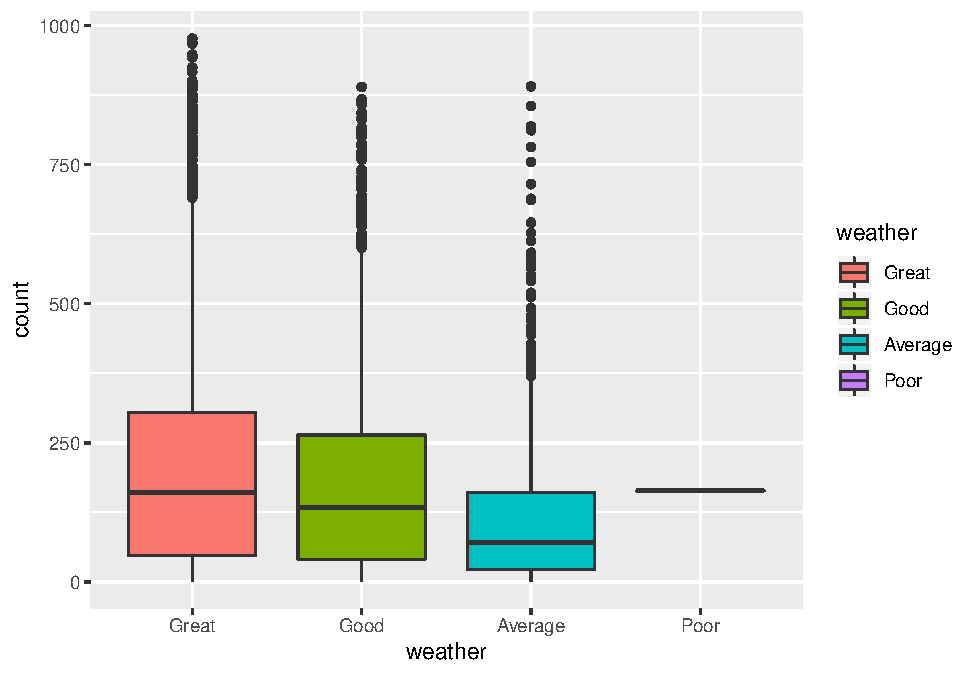
\includegraphics{BikeSharingDemand_files/figure-latex/train.mod.1.weather-1.pdf}

\newpage

\hypertarget{count-by-month}{%
\subsubsection{Count by Month}\label{count-by-month}}

The datetime column was broken out into multiple factors as well so that we could visualize the components of each date and aggregate by different dimensions of the timestamp. We felt this was also necessary due to the nature of how the train/ test data sets had been pre-split. (i.e\ldots{}with the first 19 days of the month holding the only true counts to validate our models against.)

\begin{itemize}
\tightlist
\item
  Year
\item
  Month
\item
  Day
\item
  Hour
\end{itemize}

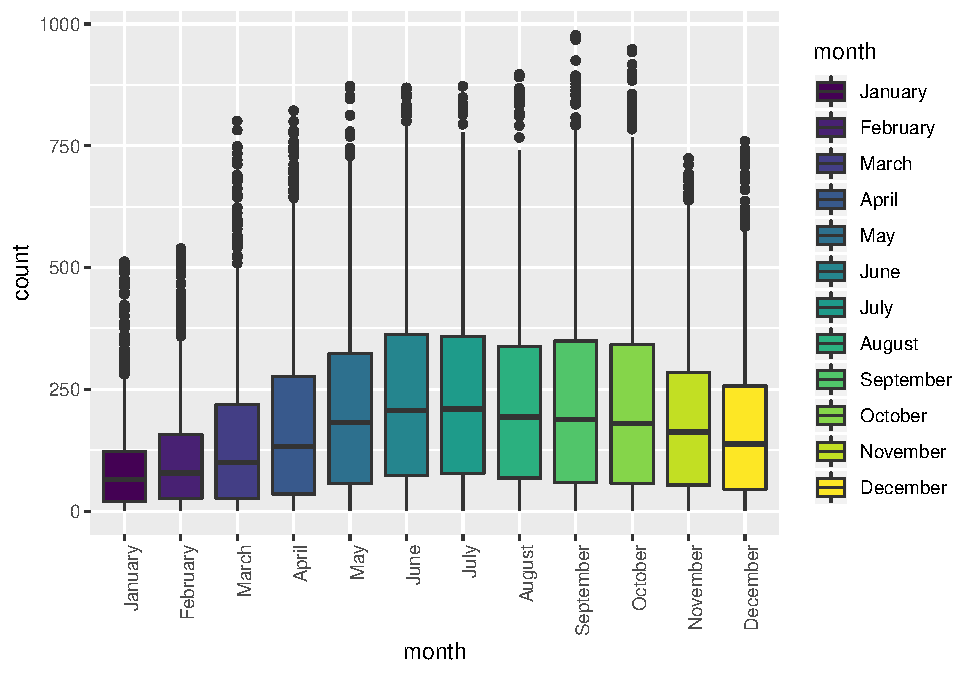
\includegraphics{BikeSharingDemand_files/figure-latex/train.mod.1.month-1.pdf}

\newpage

\hypertarget{continuous-variable-plots}{%
\subsection{Continuous Variable Plots}\label{continuous-variable-plots}}

\hypertarget{count-by-temperature}{%
\subsubsection{Count by Temperature}\label{count-by-temperature}}

The upper and lower extremes of temperature readings appear to coincide with fewer rentals.

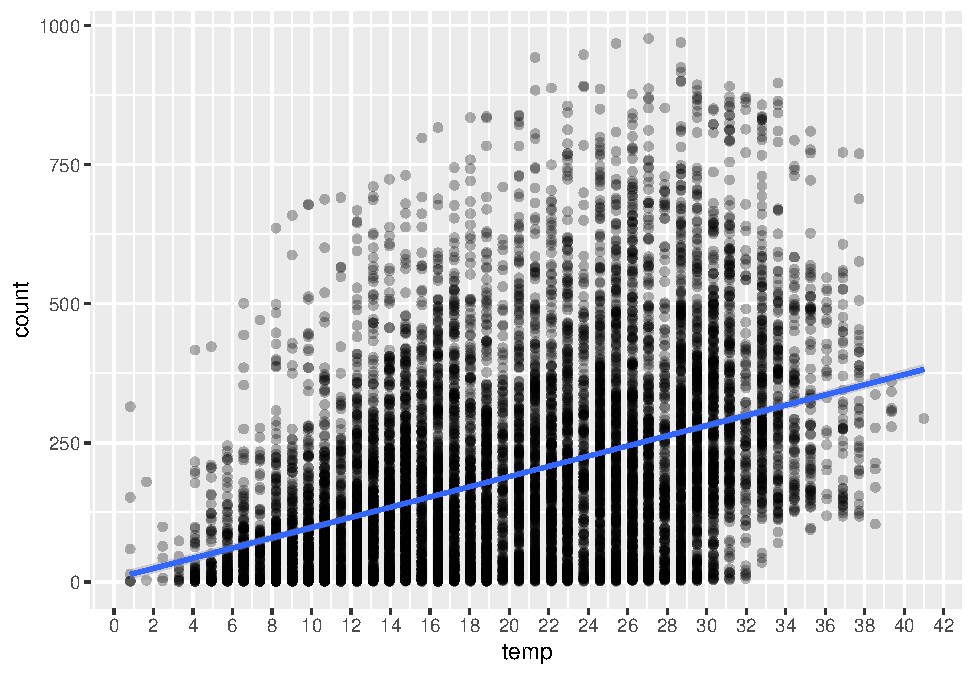
\includegraphics{BikeSharingDemand_files/figure-latex/train.mod.1.temp-1.pdf}

\newpage

\hypertarget{count-by-feels-like-temperature}{%
\subsubsection{Count by ``Feels like'' Temperature}\label{count-by-feels-like-temperature}}

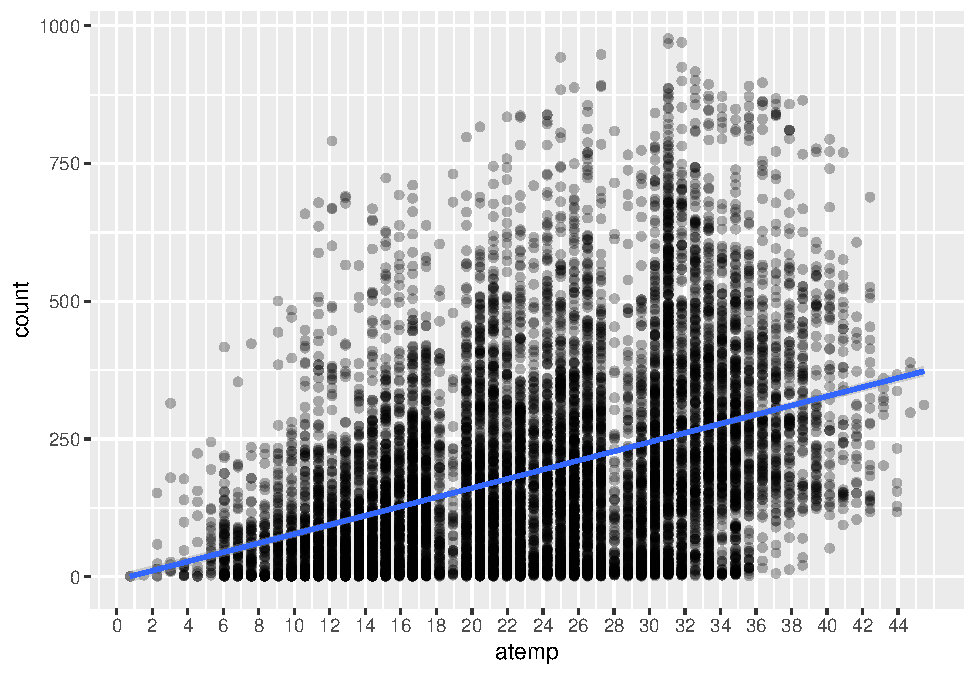
\includegraphics{BikeSharingDemand_files/figure-latex/train.mod.1.atemp-1.pdf}

\newpage

\hypertarget{count-by-wind-speed}{%
\subsubsection{Count by Wind Speed}\label{count-by-wind-speed}}

There are fewer rentals recorded as the windspeed increases beyond a certain amount.

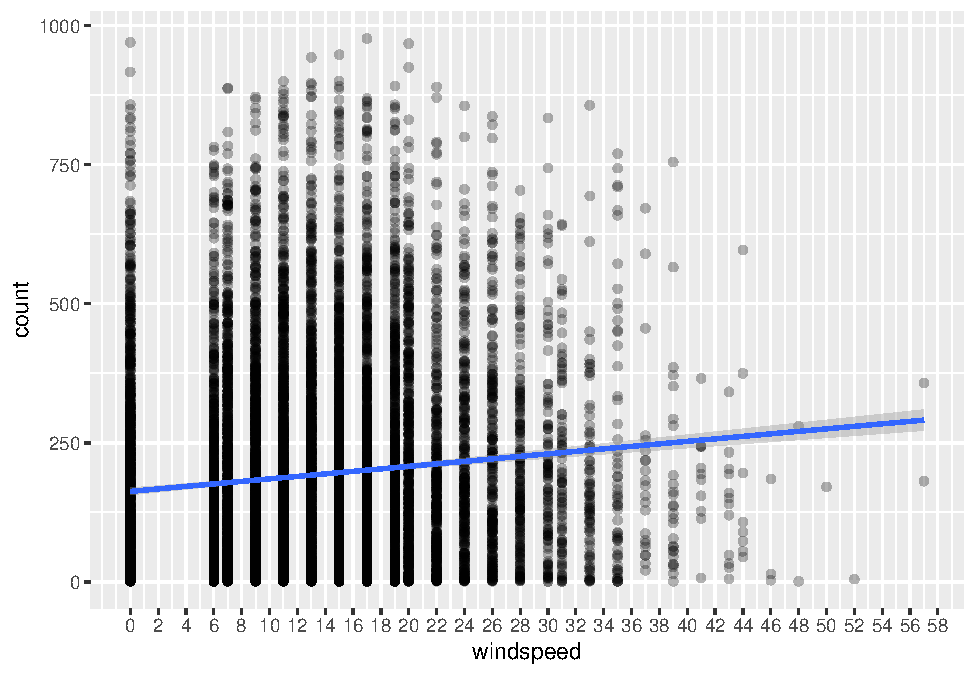
\includegraphics{BikeSharingDemand_files/figure-latex/train.mod.1.windspeed-1.pdf}

\newpage

\hypertarget{correlation-matrix}{%
\subsection{Correlation Matrix}\label{correlation-matrix}}

There are several variables with a relatively high level of covariance from the training set. The following columns should therefore be removed so as not to be picked up by any automated modelling techniques.

\begin{itemize}
\tightlist
\item
  atemp
\item
  causual
\item
  registered
\end{itemize}

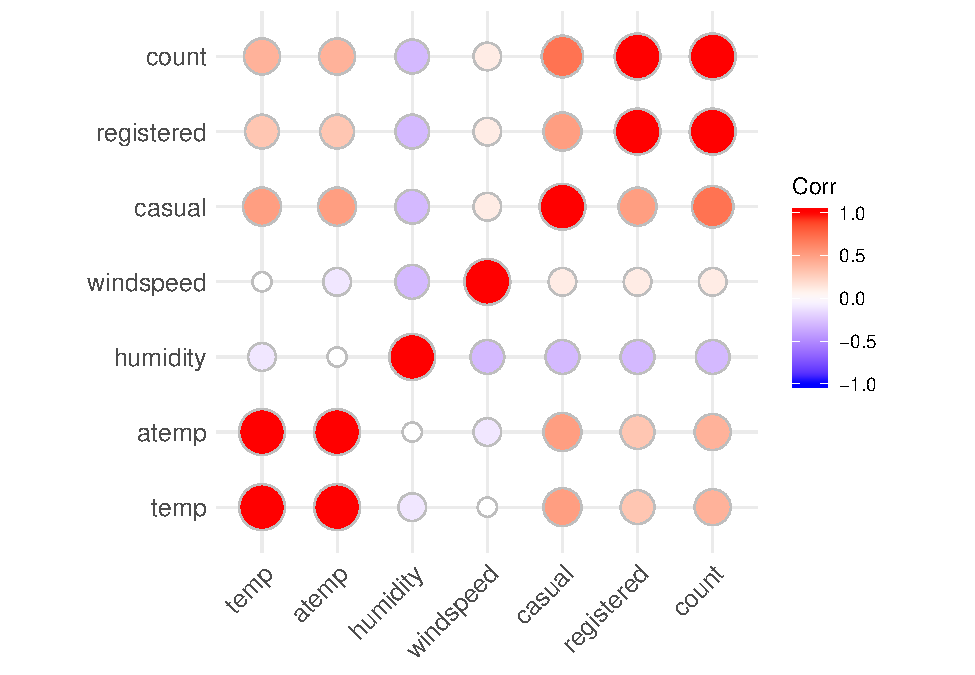
\includegraphics{BikeSharingDemand_files/figure-latex/train.mod.1.corr.matrix-1.pdf}

\newpage

\hypertarget{objective-i-analysis}{%
\section{Objective I Analysis}\label{objective-i-analysis}}

\hypertarget{question-of-interest}{%
\subsection{Question of Interest}\label{question-of-interest}}

The team be utilizing the multiple linear regression techniques we've learned up to this point in the program to predict the bike rental demand on a given date and time. The model will be evaluated on the Root Mean Squared Logarithmic Error, or RMSLE. As this data represents hourly data collected, there is an obvious time component associated with this competition. We wanted to gauge how effective multiple linear regression would be when the assumption of independence is clearly violated.

\hypertarget{model-selection}{%
\subsection{Model Selection}\label{model-selection}}

\hypertarget{lasso}{%
\subsubsection{Lasso}\label{lasso}}

We leveraged the LASSO approach to assist with variable selection for this model. Interestingly, the number of variables identified by our LASSO approach is very similar to the Stepwise approach.

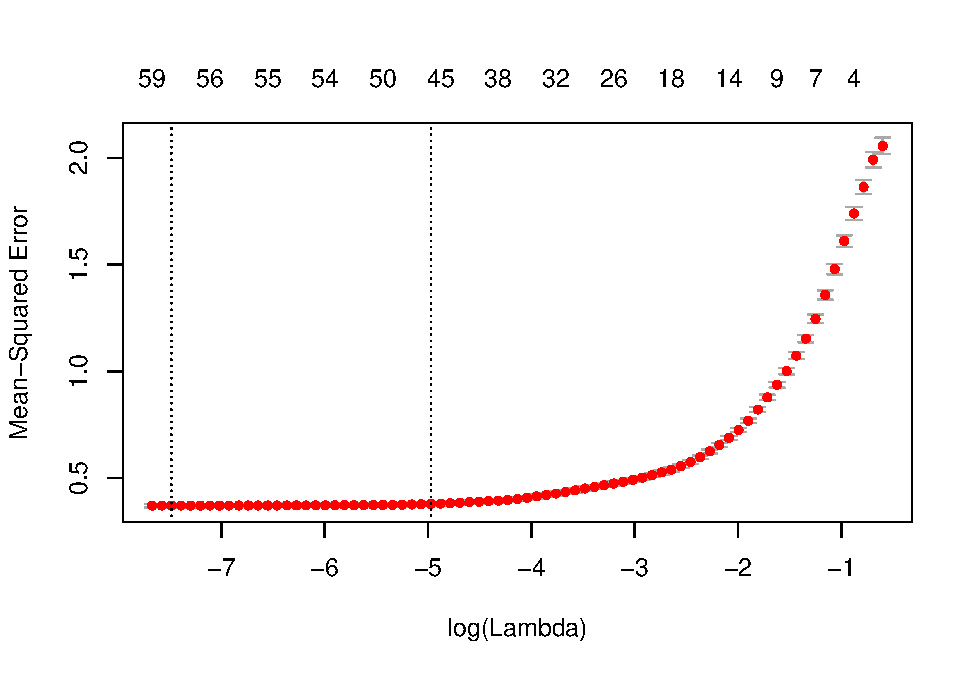
\includegraphics{BikeSharingDemand_files/figure-latex/lasso-predictors-1.pdf}

\newpage

\hypertarget{custom-variable-selection}{%
\subsubsection{Custom Variable Selection}\label{custom-variable-selection}}

We developed our custom model by adding an interactive term for month and hour based on the seasonal nature that the box plots exhibited.

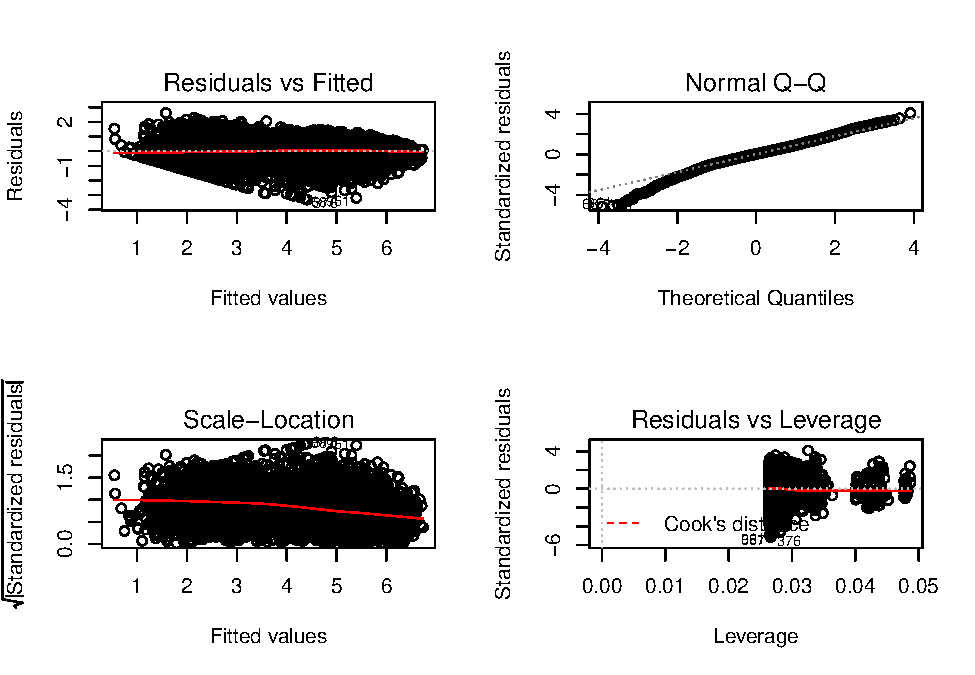
\includegraphics{BikeSharingDemand_files/figure-latex/custom-model-1.pdf} 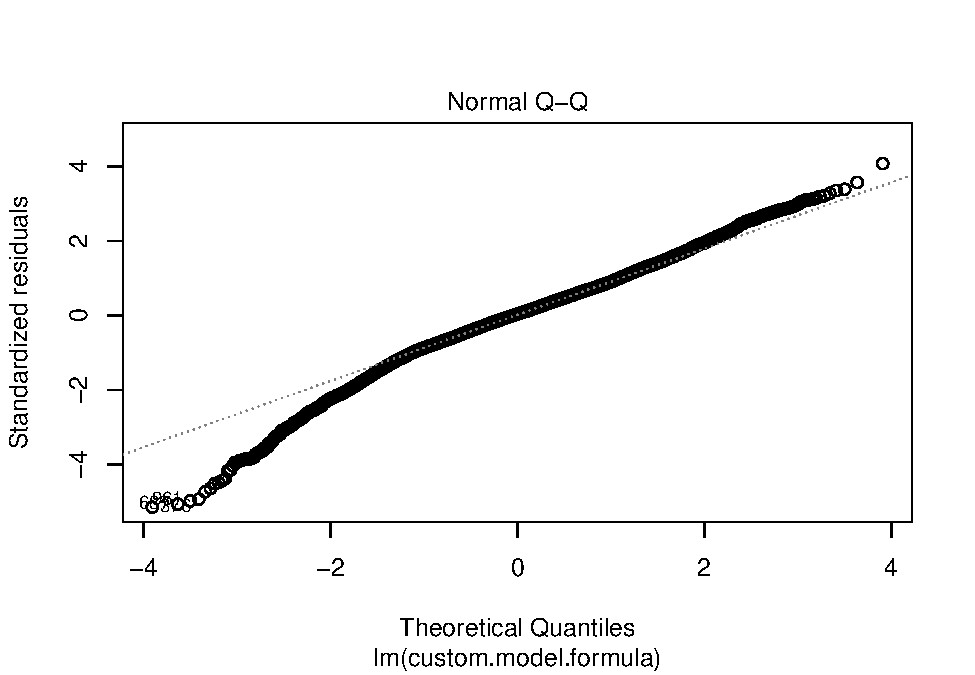
\includegraphics{BikeSharingDemand_files/figure-latex/custom-model-2.pdf}

\newpage

\hypertarget{kaggle-score}{%
\paragraph{Kaggle Score}\label{kaggle-score}}

The Root Mean Squared Logarithmic Error Loss (RMSLE) for the Kaggle submission was 0.67517 for our custom model. We scored better than around 24\% of all public submission for the competition with this technique.

\label{objective-one:custom-kaggle}

\begin{center}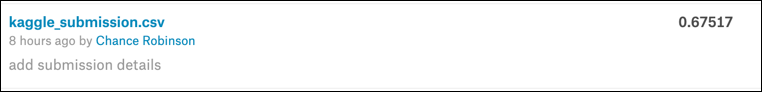
\includegraphics[width=0.9\linewidth]{./images/multiple_linear_regression_custom} \end{center}

\hypertarget{stepwise}{%
\subsubsection{Stepwise}\label{stepwise}}

Next, we leveraged the Stepwise automatic variable selection methodology. As mentioned previously, the variables selected by the Stepwise methodology are very similar to the LASSO recommendation.

\hypertarget{kaggle-score-1}{%
\paragraph{Kaggle Score}\label{kaggle-score-1}}

The Root Mean Squared Logarithmic Error Loss (RMSLE) for the Kaggle submission was 0.64765 for our stepwise model. Again, we scored better than around 24\% of all public submission for the competition with this technique, which was almost identical to that of the custom model with an interaction.

\label{objective-one:stepwise-kaggle}

\begin{center}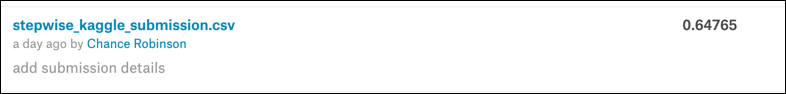
\includegraphics[width=0.9\linewidth]{./images/multiple_linear_regression_stepwise} \end{center}

\newpage

\hypertarget{model-assumptions-assessment}{%
\subsection{Model Assumptions Assessment}\label{model-assumptions-assessment}}

\begin{itemize}
\tightlist
\item
  The residual plots are approximately normal based on the QQ plot and Histogram
\item
  The log transformation of the response, in addition to extreme observation removal, has removed both outliers and observations with high leverage
\item
  The independence assumption is clearly broken due to the nature of the hourly collections. We will proceed knowing that MLR may not be the best suited model for this particular data set.
\end{itemize}

\hypertarget{comparing-competing-models}{%
\subsection{Comparing Competing Models}\label{comparing-competing-models}}

We created three models using the training bike sharing data set. All three models performed very similar across our scoring metrics and no single model stood out as the front runner. The table below summarizes the performance of the models using the adjusted R2, AIC, BIC, and RMSE:

\begin{longtable}[]{@{}lll@{}}
\toprule
Model & Adjusted R2 & AIC\tabularnewline
\midrule
\endhead
1. Custom & 0.7915 & 21642.12\tabularnewline
2. Lasso & 0.7946 & 21250.6\tabularnewline
3. Stepwise & 0.8224 & 19668.86\tabularnewline
\bottomrule
\end{longtable}

\newpage

\hypertarget{parameters}{%
\subsection{Parameters}\label{parameters}}

The following summarizes the parameters for estimates for the interaction model(custom) and the stepwise model.

\newpage

\hypertarget{stepwise-model-summary}{%
\subsubsection{Stepwise Model Summary}\label{stepwise-model-summary}}

\begin{Shaded}
\begin{Highlighting}[]
\NormalTok{stw.sm}
\end{Highlighting}
\end{Shaded}

\begin{verbatim}
## 
## Call:
## lm(formula = stw.model.formula, data = train.mod.1)
## 
## Residuals:
##      Min       1Q   Median       3Q      Max 
## -3.15355 -0.29296  0.03003  0.36343  2.28175 
## 
## Coefficients:
##                  Estimate Std. Error t value Pr(>|t|)    
## (Intercept)     3.3174555  0.0542954  61.100  < 2e-16 ***
## hour01         -0.6274075  0.0399811 -15.693  < 2e-16 ***
## hour02         -1.1359994  0.0404183 -28.106  < 2e-16 ***
## hour03         -1.6615266  0.0411443 -40.383  < 2e-16 ***
## hour04         -1.9322047  0.0414142 -46.656  < 2e-16 ***
## hour05         -0.9274850  0.0402628 -23.036  < 2e-16 ***
## hour06          0.2884532  0.0400794   7.197 6.56e-13 ***
## hour07          1.2738710  0.0399734  31.868  < 2e-16 ***
## hour08          1.9021997  0.0398896  47.687  < 2e-16 ***
## hour09          1.5748200  0.0399255  39.444  < 2e-16 ***
## hour10          1.2474375  0.0400854  31.119  < 2e-16 ***
## hour11          1.3669137  0.0403745  33.856  < 2e-16 ***
## hour12          1.5552795  0.0407026  38.211  < 2e-16 ***
## hour13          1.5299500  0.0410548  37.266  < 2e-16 ***
## hour14          1.4475331  0.0413260  35.027  < 2e-16 ***
## hour15          1.5061812  0.0414038  36.378  < 2e-16 ***
## hour16          1.7681031  0.0413060  42.805  < 2e-16 ***
## hour17          2.1811506  0.0410659  53.113  < 2e-16 ***
## hour18          2.0968370  0.0407964  51.398  < 2e-16 ***
## hour19          1.8037735  0.0403534  44.699  < 2e-16 ***
## hour20          1.5036316  0.0401264  37.472  < 2e-16 ***
## hour21          1.2442347  0.0399632  31.135  < 2e-16 ***
## hour22          1.0003851  0.0398915  25.078  < 2e-16 ***
## hour23          0.6000841  0.0398591  15.055  < 2e-16 ***
## month.L         0.6999912  0.0246473  28.400  < 2e-16 ***
## month.Q        -0.3389488  0.0425804  -7.960 1.89e-15 ***
## month.C         0.1248240  0.0217868   5.729 1.04e-08 ***
## month^4        -0.0322233  0.0226041  -1.426 0.154028    
## month^5        -0.1711829  0.0210762  -8.122 5.08e-16 ***
## month^6         0.0058324  0.0202813   0.288 0.773679    
## month^7         0.1613935  0.0204054   7.909 2.84e-15 ***
## month^8        -0.0330624  0.0201660  -1.640 0.101136    
## month^9        -0.0205400  0.0201300  -1.020 0.307577    
## month^10        0.0446766  0.0201412   2.218 0.026564 *  
## month^11       -0.0053160  0.0200316  -0.265 0.790720    
## year2012        0.4839078  0.0117932  41.033  < 2e-16 ***
## weatherGood    -0.0552311  0.0143444  -3.850 0.000119 ***
## weatherAverage -0.5515117  0.0242992 -22.697  < 2e-16 ***
## weatherPoor    -0.1034753  0.6025957  -0.172 0.863664    
## temp            0.0267535  0.0017862  14.978  < 2e-16 ***
## humidity       -0.0033135  0.0004201  -7.888 3.36e-15 ***
## workingdayYes  -0.0762112  0.0128696  -5.922 3.28e-09 ***
## windspeed      -0.0036725  0.0007753  -4.737 2.20e-06 ***
## holidayYes     -0.0632055  0.0363666  -1.738 0.082238 .  
## ---
## Signif. codes:  0 '***' 0.001 '**' 0.01 '*' 0.05 '.' 0.1 ' ' 1
## 
## Residual standard error: 0.6012 on 10736 degrees of freedom
## Multiple R-squared:  0.823,  Adjusted R-squared:  0.8223 
## F-statistic:  1161 on 43 and 10736 DF,  p-value: < 2.2e-16
\end{verbatim}

\newpage

\hypertarget{stepwise-model-confidence-intervals}{%
\subsubsection{Stepwise Model Confidence Intervals}\label{stepwise-model-confidence-intervals}}

\begin{Shaded}
\begin{Highlighting}[]
\NormalTok{stw.model.conf}
\end{Highlighting}
\end{Shaded}

\begin{verbatim}
##                       2.5 %       97.5 %
## (Intercept)     3.211026394  3.423884533
## hour01         -0.705777933 -0.549037038
## hour02         -1.215226626 -1.056772119
## hour03         -1.742176911 -1.580876202
## hour04         -2.013384298 -1.851025149
## hour05         -1.006407588 -0.848562369
## hour06          0.209890114  0.367016273
## hour07          1.195515864  1.352226204
## hour08          1.824008596  1.980390741
## hour09          1.496558675  1.653081418
## hour10          1.168862680  1.326012291
## hour11          1.287772330  1.446055168
## hour12          1.475494788  1.635064118
## hour13          1.449474949  1.610425000
## hour14          1.366526484  1.528539618
## hour15          1.425022148  1.587340244
## hour16          1.687135770  1.849070459
## hour17          2.100653854  2.261647266
## hour18          2.016868484  2.176805446
## hour19          1.724673301  1.882873603
## hour20          1.424976440  1.582286771
## hour21          1.165899502  1.322569880
## hour22          0.922190315  1.078579819
## hour23          0.521952963  0.678215327
## month.L         0.651677911  0.748304457
## month.Q        -0.422414228 -0.255483406
## month.C         0.082117898  0.167530202
## month^4        -0.076531522  0.012085007
## month^5        -0.212496092 -0.129869713
## month^6        -0.033922711  0.045587412
## month^7         0.121395096  0.201391945
## month^8        -0.072591494  0.006466684
## month^9        -0.059998566  0.018918535
## month^10        0.005196073  0.084157154
## month^11       -0.044581694  0.033949624
## year2012        0.460791009  0.507024554
## weatherGood    -0.083348733 -0.027113558
## weatherAverage -0.599142667 -0.503880774
## weatherPoor    -1.284674358  1.077723669
## temp            0.023252232  0.030254717
## humidity       -0.004136865 -0.002490104
## workingdayYes  -0.101438121 -0.050984345
## windspeed      -0.005192272 -0.002152635
## holidayYes     -0.134490754  0.008079730
\end{verbatim}

\newpage

\hypertarget{model-interpretation}{%
\subsection{Model Interpretation}\label{model-interpretation}}

For the Stepwise model, keeping the temp and humidity constant a unit increase in windspeed is associated with a multiplicative change of 0.997 units in median of counts. The 95\% confidence interval for the multiplicative change is = (0.994, .998)

Keeping the temp and windspeed constant a unit increase in humidity is associated with a multiplicative change of 0.997 unit in median of counts. The 95\% confidence interval for the multiplicative change is =(0.996, .998)

Keeping humidity and temperature constant a unit change in temperature is associated with a multiplicative change of 1.03 units in median of counts. The 95\% confidence interval for the multiplicative change is = (1.02, 1.031)

\textbf{Stepwise Model}

\begin{align}
\mu \lbrace log(count) \rbrace = \hat{\beta_0} + \hat{\beta_1} (hour) +  \hat{\beta_2} (month) + 
\nonumber\\
\hat{\beta_3} (year) + \hat{\beta_4} (weather) +  \hat{\beta_5} (temp) + \hat{\beta_6} (humidity) +
\nonumber\\
\hat{\beta_7} (workingday) +  \hat{\beta_8} (windspeed) + \hat{\beta_9} (holiday)\label{eq:Stepwise}
\end{align}

\hypertarget{conclusion}{%
\subsection{Conclusion}\label{conclusion}}

To conclude, based on the initial EDA, it was identified that a log-linear model was a be better fit for Multiple Linear Regression. Also, once the outliers were identified and excluded, we ran LASSO, stepwise and custom model selection on the dataset. As we can see from the above sections, the results from the stepwise and custom models were very close. We find that the stepwise performed slightly better than the custom and LASSO models with the lowest standard error measures (AIC = 19668, BIC = 19996 and RMSE = 0.599).

\newpage

\hypertarget{objective-ii-analysis}{%
\section{Objective II Analysis}\label{objective-ii-analysis}}

\hypertarget{question-of-interest-1}{%
\subsection{Question of Interest}\label{question-of-interest-1}}

As the independence assumption from Objective I appears to have been violated, the team wanted to apply the time series analysis techniques we've learned up to this point in the MSDS program in an attempt to address the issue. The primary goal was to compare and contrast the performance of auto arima models versus those that we modeled on our own.

Additionally, we wanted to compare the Kaggle submission to that from Objective I to see if our predictions were better or worse than from the prior objective.

\hypertarget{data-preperation}{%
\subsection{Data Preperation}\label{data-preperation}}

As the data had been pre-split monthly, we needed to make our predictions from the 20th of each month and on for each year of recorded bike rentals. (2011 and 2012) The approach has been summarized with the steps below.

\begin{enumerate}
\def\labelenumi{\arabic{enumi}.}
\item
  Log the response variable
\item
  Loop through years
\item
  Loop through months
\item
  Fit AR model
\item
  Forcast x number of observations based on the number of rows from test data frame and impute the count from the time series forecast
\end{enumerate}

\newpage

\hypertarget{comparing-competing-models-1}{%
\subsection{Comparing Competing Models}\label{comparing-competing-models-1}}

\hypertarget{auto-arima}{%
\subsubsection{Auto Arima}\label{auto-arima}}

\begin{verbatim}
## 
##  Ljung-Box test
## 
## data:  Residuals from ARIMA(4,0,4) with non-zero mean
## Q* = 10.049, df = 3, p-value = 0.01816
## 
## Model df: 9.   Total lags used: 12
\end{verbatim}

\begin{figure}[htbp]

{\centering 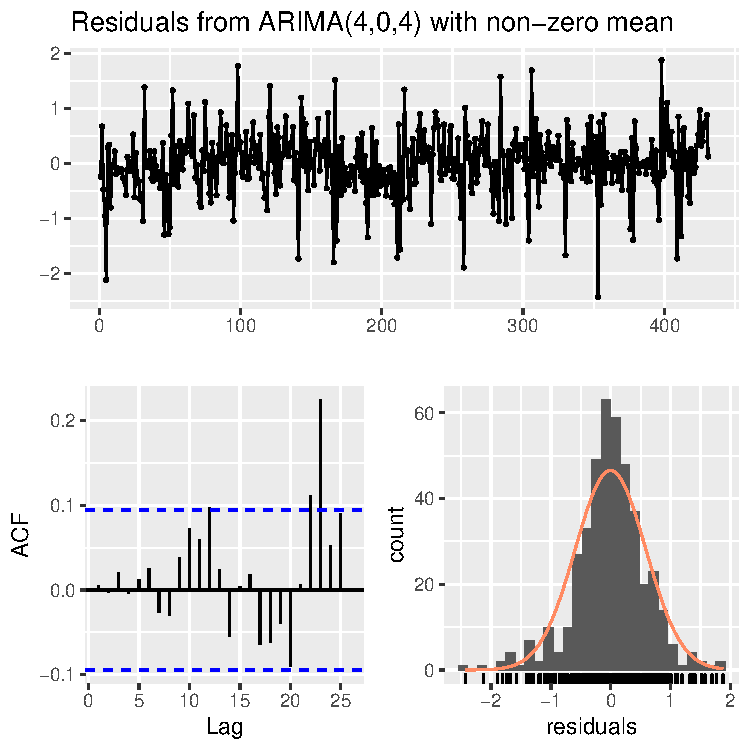
\includegraphics[width=0.45\linewidth]{BikeSharingDemand_files/figure-latex/auto-arima-plot-1-1} 

}

\caption{Auto Arima Residual Plots}\label{fig:auto-arima-plot-1}
\end{figure}

\begin{figure}[htbp]

{\centering 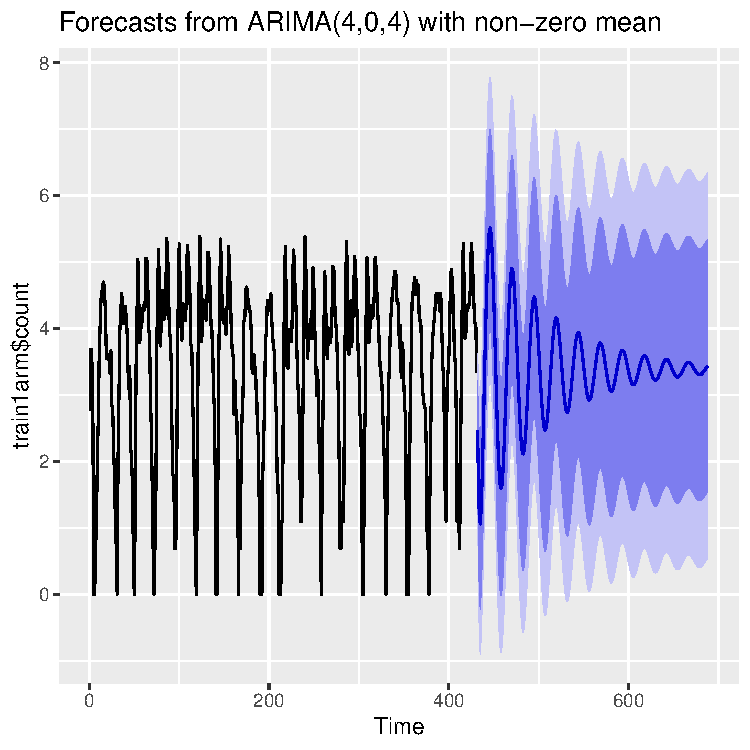
\includegraphics[width=0.45\linewidth]{BikeSharingDemand_files/figure-latex/auto-arima-plot-2-1} 

}

\caption{Auto Arima Forecasts}\label{fig:auto-arima-plot-2}
\end{figure}

\newpage

\hypertarget{auto-regression}{%
\subsubsection{Auto Regression}\label{auto-regression}}

\begin{verbatim}
## 
##  Ljung-Box test
## 
## data:  Residuals from ARIMA(25,0,0) with non-zero mean
## Q* = 11.131, df = 3, p-value = 0.01104
## 
## Model df: 26.   Total lags used: 29
\end{verbatim}

\begin{figure}[htbp]

{\centering 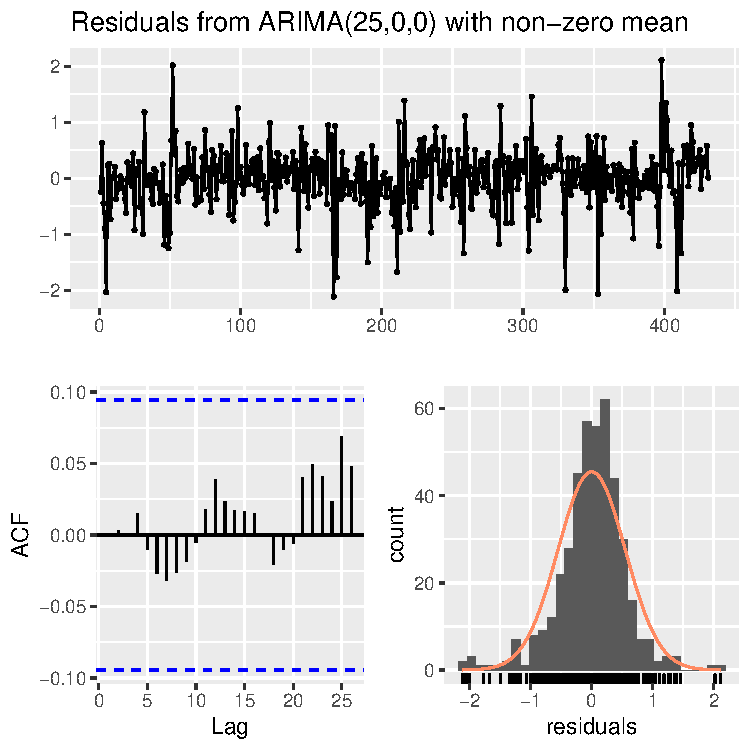
\includegraphics[width=0.45\linewidth]{BikeSharingDemand_files/figure-latex/arima-25-plot-1-1} 

}

\caption{Arima (25) Residual Plots}\label{fig:arima-25-plot-1}
\end{figure}

\begin{figure}[htbp]

{\centering 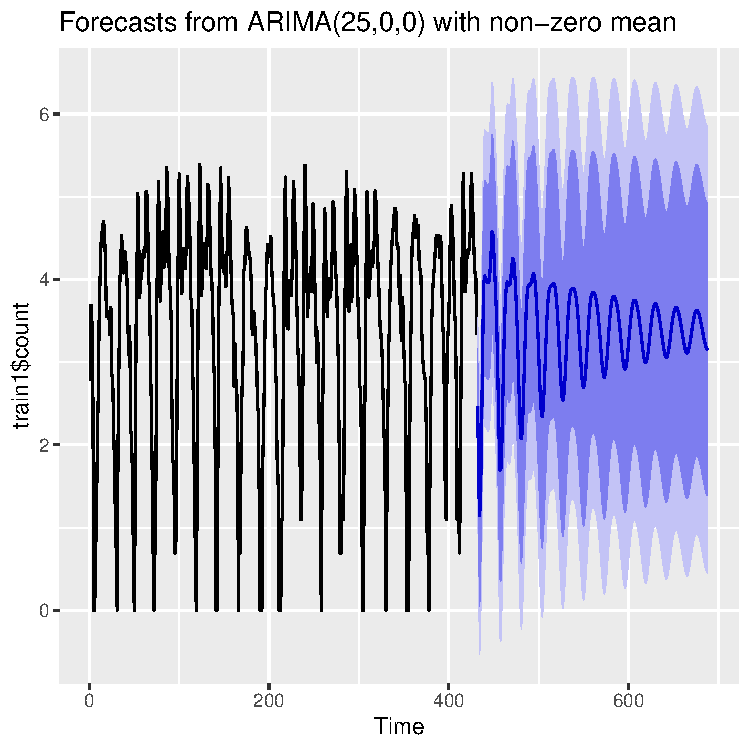
\includegraphics[width=0.45\linewidth]{BikeSharingDemand_files/figure-latex/arima-25-plot-2-1} 

}

\caption{Arima (25) Forecasts}\label{fig:arima-25-plot-2}
\end{figure}

\newpage

\hypertarget{accuracy-metrics}{%
\subsubsection{Accuracy Metrics}\label{accuracy-metrics}}

The accuracy metrics appear to go in favor of the AR25 model. In some year/ month combinations the difference was more obvious and was more reason to utilize the AR25 method.

\begin{table}[H]
\centering
\begin{tabular}{lrrr}
\toprule
Model & RMSLE & AIC & Variance\\
\midrule
ARIMA & 0.2418941 & 791.5698 & 0.3541476\\
AR25 & 0.2265693 & 768.3810 & 0.3025818\\
\bottomrule
\end{tabular}
\end{table}

\newpage

\hypertarget{kaggle-score-2}{%
\paragraph{Kaggle Score}\label{kaggle-score-2}}

The Root Mean Squared Logarithmic Error Loss (RMSLE) for the Kaggle submission was 1.01847 for our AR25 model. We scored better than only 14.48\% of all public submission for the competition which was considerably worse than our score from all of the multiple linear regression models above.

\label{objective-two:ar25-kaggle}

\begin{center}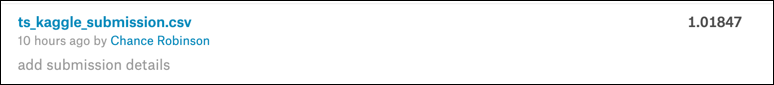
\includegraphics[width=0.9\linewidth]{./images/time_series_ar25} \end{center}

\hypertarget{model-assumption-assessment}{%
\subsection{Model Assumption Assessment}\label{model-assumption-assessment}}

Both the ARIMA and AR 25 models showed a constant mean and variance for the timespan of the observations. The auto-correlations however were noticeably better for the AR 25 graph. The error terms were also slightly improved which is the reason we elected to not go with the automated selection approach.

\begin{itemize}
\tightlist
\item
  Constant Mean
\item
  Constant Variance
\item
  Constant auto-correlations
\end{itemize}

\hypertarget{conclusion-1}{%
\subsection{Conclusion}\label{conclusion-1}}

Although the data set was found to be serially correlated, ultimately applying time series techniques was not enough to improve our RMSLE above and beyond the multiple linear regression techniques from objective one. Again, this likely had more to do with the fact that we were attempting to predict future observations 10 plus days in advance on a monthly basis. And with the seasonal nature of our hourly observations, the accuracy of the prediction became less accurate over time and showed a regression to the mean after only a few days' worth of predictions. The immediate observations however, within 24 to 48 hours, visually at least showed much better predictive trends.

\newpage

\hypertarget{appendix}{%
\section{Appendix}\label{appendix}}

\hypertarget{code}{%
\subsection{Code}\label{code}}

\hypertarget{r-code-for-objective-i}{%
\subsubsection{R Code For Objective I}\label{r-code-for-objective-i}}

\begin{Shaded}
\begin{Highlighting}[]
\CommentTok{### Library Imports}
\KeywordTok{library}\NormalTok{(tidyverse)}
\CommentTok{# Date manipulation}
\KeywordTok{library}\NormalTok{(lubridate)}
\CommentTok{# Plotting}
\KeywordTok{library}\NormalTok{(olsrr)}
\CommentTok{# RMLSE}
\KeywordTok{library}\NormalTok{(MLmetrics)}


\CommentTok{### Load the csv data}
\NormalTok{train <-}\StringTok{ }\KeywordTok{read_csv}\NormalTok{(}\StringTok{'../../../data/train.csv'}\NormalTok{)}
\NormalTok{test <-}\StringTok{ }\KeywordTok{read_csv}\NormalTok{(}\StringTok{'../../../data/test.csv'}\NormalTok{)}

\CommentTok{### Identify Dimensions}

\NormalTok{no_of_rows_trn <-}\StringTok{ }\KeywordTok{dim}\NormalTok{(train)[}\DecValTok{1}\NormalTok{]}
\NormalTok{no_of_rows_tst <-}\StringTok{ }\KeywordTok{dim}\NormalTok{(test)[}\DecValTok{1}\NormalTok{]}

\NormalTok{no_of_cols_trn <-}\StringTok{ }\KeywordTok{dim}\NormalTok{(train)[}\DecValTok{2}\NormalTok{]}
\NormalTok{no_of_cols_tst <-}\StringTok{ }\KeywordTok{dim}\NormalTok{(test)[}\DecValTok{2}\NormalTok{]}

\CommentTok{# no_of_rows_trn}
\CommentTok{# no_of_rows_tst}
\CommentTok{# }
\CommentTok{# no_of_cols_trn}
\CommentTok{# no_of_cols_tst}

\CommentTok{### Missing Data (Both)}

\CommentTok{# train}
\KeywordTok{any}\NormalTok{(}\KeywordTok{is.na}\NormalTok{(train))}

\CommentTok{# test}
\KeywordTok{any}\NormalTok{(}\KeywordTok{is.na}\NormalTok{(test))}


\CommentTok{### Log the response variable}
\NormalTok{train}\OperatorTok{$}\NormalTok{count <-}\StringTok{ }\KeywordTok{log}\NormalTok{(train}\OperatorTok{$}\NormalTok{count)}


\CommentTok{### Factors}
\NormalTok{train}\OperatorTok{$}\NormalTok{season <-}\StringTok{ }\KeywordTok{factor}\NormalTok{(train}\OperatorTok{$}\NormalTok{season, }\DataTypeTok{labels =} \KeywordTok{c}\NormalTok{(}\StringTok{"Spring"}\NormalTok{, }\StringTok{"Summer"}\NormalTok{, }\StringTok{"Fall"}\NormalTok{, }\StringTok{"Winter"}\NormalTok{))}
\NormalTok{test}\OperatorTok{$}\NormalTok{season <-}\StringTok{ }\KeywordTok{factor}\NormalTok{(test}\OperatorTok{$}\NormalTok{season, }\DataTypeTok{labels =} \KeywordTok{c}\NormalTok{(}\StringTok{"Spring"}\NormalTok{, }\StringTok{"Summer"}\NormalTok{, }\StringTok{"Fall"}\NormalTok{, }\StringTok{"Winter"}\NormalTok{))}

\KeywordTok{table}\NormalTok{(train}\OperatorTok{$}\NormalTok{season)}

\NormalTok{train}\OperatorTok{$}\NormalTok{holiday <-}\StringTok{ }\KeywordTok{factor}\NormalTok{(train}\OperatorTok{$}\NormalTok{holiday, }\DataTypeTok{labels =} \KeywordTok{c}\NormalTok{(}\StringTok{"No"}\NormalTok{, }\StringTok{"Yes"}\NormalTok{))}
\NormalTok{test}\OperatorTok{$}\NormalTok{holiday <-}\StringTok{ }\KeywordTok{factor}\NormalTok{(test}\OperatorTok{$}\NormalTok{holiday, }\DataTypeTok{labels =} \KeywordTok{c}\NormalTok{(}\StringTok{"No"}\NormalTok{, }\StringTok{"Yes"}\NormalTok{))}

\KeywordTok{table}\NormalTok{(train}\OperatorTok{$}\NormalTok{holiday)}

\NormalTok{train}\OperatorTok{$}\NormalTok{workingday <-}\StringTok{ }\KeywordTok{factor}\NormalTok{(train}\OperatorTok{$}\NormalTok{workingday, }\DataTypeTok{labels =} \KeywordTok{c}\NormalTok{(}\StringTok{"No"}\NormalTok{, }\StringTok{"Yes"}\NormalTok{))}
\NormalTok{test}\OperatorTok{$}\NormalTok{workingday <-}\StringTok{ }\KeywordTok{factor}\NormalTok{(test}\OperatorTok{$}\NormalTok{workingday, }\DataTypeTok{labels =} \KeywordTok{c}\NormalTok{(}\StringTok{"No"}\NormalTok{, }\StringTok{"Yes"}\NormalTok{))}

\KeywordTok{table}\NormalTok{(train}\OperatorTok{$}\NormalTok{workingday)}

\NormalTok{train}\OperatorTok{$}\NormalTok{weather <-}\StringTok{ }\KeywordTok{factor}\NormalTok{(train}\OperatorTok{$}\NormalTok{weather, }\DataTypeTok{labels =} \KeywordTok{c}\NormalTok{(}\StringTok{"Great"}\NormalTok{, }\StringTok{"Good"}\NormalTok{, }\StringTok{"Average"}\NormalTok{, }\StringTok{"Poor"}\NormalTok{))}
\NormalTok{test}\OperatorTok{$}\NormalTok{weather <-}\StringTok{ }\KeywordTok{factor}\NormalTok{(test}\OperatorTok{$}\NormalTok{weather, }\DataTypeTok{labels =} \KeywordTok{c}\NormalTok{(}\StringTok{"Great"}\NormalTok{, }\StringTok{"Good"}\NormalTok{, }\StringTok{"Average"}\NormalTok{, }\StringTok{"Poor"}\NormalTok{))}

\KeywordTok{table}\NormalTok{(train}\OperatorTok{$}\NormalTok{weather)}


\CommentTok{### Split Date-Time (Both)}
\NormalTok{train <-}\StringTok{ }\NormalTok{train }\OperatorTok
\StringTok{  }\KeywordTok{mutate}\NormalTok{(}\DataTypeTok{year =} \KeywordTok{as.factor}\NormalTok{(}\KeywordTok{format}\NormalTok{(datetime, }\DataTypeTok{format =} \StringTok{"%Y"}\NormalTok{)), }
         \DataTypeTok{month =} \KeywordTok{as.numeric}\NormalTok{(}\KeywordTok{format}\NormalTok{(datetime, }\DataTypeTok{format =} \StringTok{"%m"}\NormalTok{)), }
         \DataTypeTok{day =} \KeywordTok{as.factor}\NormalTok{(}\KeywordTok{format}\NormalTok{(datetime, }\DataTypeTok{format =} \StringTok{"%d"}\NormalTok{)),}
         \DataTypeTok{hour =} \KeywordTok{as.factor}\NormalTok{(}\KeywordTok{format}\NormalTok{(datetime, }\DataTypeTok{format =} \StringTok{"%H"}\NormalTok{)))}

\NormalTok{test <-}\StringTok{ }\NormalTok{test }\OperatorTok
\StringTok{  }\KeywordTok{mutate}\NormalTok{(}\DataTypeTok{year =} \KeywordTok{as.factor}\NormalTok{(}\KeywordTok{format}\NormalTok{(datetime, }\DataTypeTok{format =} \StringTok{"%Y"}\NormalTok{)), }
         \DataTypeTok{month =} \KeywordTok{as.numeric}\NormalTok{(}\KeywordTok{format}\NormalTok{(datetime, }\DataTypeTok{format =} \StringTok{"%m"}\NormalTok{)), }
         \DataTypeTok{day =} \KeywordTok{as.factor}\NormalTok{(}\KeywordTok{format}\NormalTok{(datetime, }\DataTypeTok{format =} \StringTok{"%d"}\NormalTok{)),}
         \DataTypeTok{hour =} \KeywordTok{as.factor}\NormalTok{(}\KeywordTok{format}\NormalTok{(datetime, }\DataTypeTok{format =} \StringTok{"%H"}\NormalTok{)))}



\CommentTok{### Convert Months to Ordered Factor (Both)}
\NormalTok{train}\OperatorTok{$}\NormalTok{month <-}\KeywordTok{month}\NormalTok{(train}\OperatorTok{$}\NormalTok{datetime, }\DataTypeTok{label =} \OtherTok{TRUE}\NormalTok{, }\DataTypeTok{abbr =} \OtherTok{FALSE}\NormalTok{)}
\NormalTok{test}\OperatorTok{$}\NormalTok{month <-}\KeywordTok{month}\NormalTok{(test}\OperatorTok{$}\NormalTok{datetime, }\DataTypeTok{label =} \OtherTok{TRUE}\NormalTok{, }\DataTypeTok{abbr =} \OtherTok{FALSE}\NormalTok{)}



\CommentTok{### Outlier}
\NormalTok{outliers <-}\StringTok{ }\NormalTok{train[   train}\OperatorTok{$}\NormalTok{count }\OperatorTok{<}\StringTok{ }\KeywordTok{median}\NormalTok{(train}\OperatorTok{$}\NormalTok{count) }\OperatorTok{-}\StringTok{ }\NormalTok{(}\KeywordTok{sd}\NormalTok{(train}\OperatorTok{$}\NormalTok{count) }\OperatorTok{*}\StringTok{ }\DecValTok{3}\NormalTok{), ]}
\CommentTok{# outliers}

\NormalTok{train }\OperatorTok
\StringTok{  }\KeywordTok{group_by}\NormalTok{(month) }\OperatorTok
\StringTok{  }\KeywordTok{summarize}\NormalTok{(}\DataTypeTok{mean =} \KeywordTok{mean}\NormalTok{(count), }\DataTypeTok{sd =} \KeywordTok{sd}\NormalTok{(count), }\DataTypeTok{median =} \KeywordTok{median}\NormalTok{(count), }\DataTypeTok{observations =} \KeywordTok{n}\NormalTok{())}


\CommentTok{# remove outliers}
\NormalTok{train <-}\StringTok{ }\NormalTok{train }\OperatorTok
\StringTok{  }\KeywordTok{filter}\NormalTok{(}\OperatorTok{!}\NormalTok{datetime }\OperatorTok\StringTok{ }\NormalTok{outliers}\OperatorTok{$}\NormalTok{datetime)}

\CommentTok{# Extreme Observation}
\CommentTok{# train[5555, ] # 2012-01-09 18:00:00}
\NormalTok{train <-}\StringTok{ }\NormalTok{train }\OperatorTok
\StringTok{  }\KeywordTok{filter}\NormalTok{(datetime }\OperatorTok{!=}\StringTok{ '2012-01-09 18:00:00'}\NormalTok{)}



\CommentTok{### Model Fitting}

\CommentTok{### Custom Model}
\NormalTok{model.base.formula =}\StringTok{ }\NormalTok{count }\OperatorTok{~}\StringTok{ }\NormalTok{weather }\OperatorTok{+}\StringTok{ }
\StringTok{                             }\NormalTok{windspeed }\OperatorTok{+}\StringTok{ }
\StringTok{                             }\NormalTok{temp }\OperatorTok{+}\StringTok{ }
\StringTok{                             }\NormalTok{month }\OperatorTok{+}
\StringTok{                             }\NormalTok{hour }\OperatorTok{+}
\StringTok{                             }\NormalTok{month}\OperatorTok{:}\NormalTok{hour}
  
  \CommentTok{# datetime}


\NormalTok{model  <-}\StringTok{ }\KeywordTok{lm}\NormalTok{(}\DataTypeTok{formula =}\NormalTok{ model.base.formula, }\DataTypeTok{data =}\NormalTok{ train)}

\KeywordTok{plot}\NormalTok{(model)}

\KeywordTok{summary}\NormalTok{(model)}

\KeywordTok{ols_plot_resid_lev}\NormalTok{(model)}



\CommentTok{### Stepwise Model}
\NormalTok{train.mod}\FloatTok{.1}\OperatorTok{$}\NormalTok{datetime <-}\StringTok{ }\OtherTok{NULL}
\NormalTok{train.mod}\FloatTok{.1}\OperatorTok{$}\NormalTok{datetime <-}\StringTok{ }\OtherTok{NULL}

\CommentTok{# Fit the model with all parameters}
\NormalTok{fit1 <-}\StringTok{ }\KeywordTok{lm}\NormalTok{(count }\OperatorTok{~}\StringTok{ }\NormalTok{., }\DataTypeTok{data=}\NormalTok{train.mod}\FloatTok{.1}\NormalTok{)}
\CommentTok{# Fit the model with only 1 parameter}
\NormalTok{fit2 <-}\StringTok{ }\KeywordTok{lm}\NormalTok{(count }\OperatorTok{~}\StringTok{ }\DecValTok{1}\NormalTok{, }\DataTypeTok{data=}\NormalTok{train.mod}\FloatTok{.1}\NormalTok{)}


\CommentTok{# stw.model <- stepAIC(fit2,direction="both",scope=list(upper=fit1,lower=fit2))}
\CommentTok{# summary(stw.model)}

\NormalTok{stw.model.formula <-}\StringTok{ }\NormalTok{count }\OperatorTok{~}\StringTok{ }\NormalTok{hour }\OperatorTok{+}\StringTok{ }\NormalTok{month }\OperatorTok{+}\StringTok{ }\NormalTok{year }\OperatorTok{+}\StringTok{ }\NormalTok{weather }\OperatorTok{+}\StringTok{ }\NormalTok{temp }\OperatorTok{+}\StringTok{ }\NormalTok{humidity }\OperatorTok{+}\StringTok{ }
\StringTok{  }\NormalTok{workingday }\OperatorTok{+}\StringTok{ }\NormalTok{windspeed }\OperatorTok{+}\StringTok{ }\NormalTok{holiday}

\NormalTok{stw.model <-}\StringTok{ }\KeywordTok{lm}\NormalTok{(stw.model.formula,}
               \DataTypeTok{data =}\NormalTok{ train.mod}\FloatTok{.1}\NormalTok{)}

\NormalTok{stw.sm <-}\StringTok{ }\KeywordTok{summary}\NormalTok{(stw.model)}
\NormalTok{stw.sm.coe <-}\StringTok{ }\NormalTok{stw.sm}\OperatorTok{$}\NormalTok{coefficients}

\CommentTok{# get the CIs for the coefficients}
\NormalTok{stw.model.conf <-}\StringTok{ }\KeywordTok{confint}\NormalTok{(stw.model)}
\end{Highlighting}
\end{Shaded}

\newpage

\hypertarget{r-code-for-objective-ii}{%
\subsubsection{R Code For Objective II}\label{r-code-for-objective-ii}}

\begin{Shaded}
\begin{Highlighting}[]
\CommentTok{### Library Imports}

\KeywordTok{library}\NormalTok{(tidyverse)}
\CommentTok{# Date manipulation}
\KeywordTok{library}\NormalTok{(lubridate)}
\CommentTok{# RMLSE}
\KeywordTok{library}\NormalTok{(MLmetrics)}
\CommentTok{# Time Series Analysis}
\KeywordTok{library}\NormalTok{(tseries)}
\KeywordTok{library}\NormalTok{(forecast)}


\CommentTok{### Load the csv data}
\NormalTok{train <-}\StringTok{ }\KeywordTok{read_csv}\NormalTok{(}\StringTok{'../../../data/train.csv'}\NormalTok{)}
\NormalTok{test <-}\StringTok{ }\KeywordTok{read_csv}\NormalTok{(}\StringTok{'../../../data/test.csv'}\NormalTok{)}


\CommentTok{### Categorical Factors}
\NormalTok{train}\OperatorTok{$}\NormalTok{season <-}\StringTok{ }\KeywordTok{factor}\NormalTok{(train}\OperatorTok{$}\NormalTok{season, }\DataTypeTok{labels =} \KeywordTok{c}\NormalTok{(}\StringTok{"Spring"}\NormalTok{, }\StringTok{"Summer"}\NormalTok{, }\StringTok{"Fall"}\NormalTok{, }\StringTok{"Winter"}\NormalTok{))}
\NormalTok{test}\OperatorTok{$}\NormalTok{season <-}\StringTok{ }\KeywordTok{factor}\NormalTok{(test}\OperatorTok{$}\NormalTok{season, }\DataTypeTok{labels =} \KeywordTok{c}\NormalTok{(}\StringTok{"Spring"}\NormalTok{, }\StringTok{"Summer"}\NormalTok{, }\StringTok{"Fall"}\NormalTok{, }\StringTok{"Winter"}\NormalTok{))}

\KeywordTok{table}\NormalTok{(train}\OperatorTok{$}\NormalTok{season)}

\NormalTok{train}\OperatorTok{$}\NormalTok{holiday <-}\StringTok{ }\KeywordTok{factor}\NormalTok{(train}\OperatorTok{$}\NormalTok{holiday, }\DataTypeTok{labels =} \KeywordTok{c}\NormalTok{(}\StringTok{"No"}\NormalTok{, }\StringTok{"Yes"}\NormalTok{))}
\NormalTok{test}\OperatorTok{$}\NormalTok{holiday <-}\StringTok{ }\KeywordTok{factor}\NormalTok{(test}\OperatorTok{$}\NormalTok{holiday, }\DataTypeTok{labels =} \KeywordTok{c}\NormalTok{(}\StringTok{"No"}\NormalTok{, }\StringTok{"Yes"}\NormalTok{))}

\KeywordTok{table}\NormalTok{(train}\OperatorTok{$}\NormalTok{holiday)}

\NormalTok{train}\OperatorTok{$}\NormalTok{workingday <-}\StringTok{ }\KeywordTok{factor}\NormalTok{(train}\OperatorTok{$}\NormalTok{workingday, }\DataTypeTok{labels =} \KeywordTok{c}\NormalTok{(}\StringTok{"No"}\NormalTok{, }\StringTok{"Yes"}\NormalTok{))}
\NormalTok{test}\OperatorTok{$}\NormalTok{workingday <-}\StringTok{ }\KeywordTok{factor}\NormalTok{(test}\OperatorTok{$}\NormalTok{workingday, }\DataTypeTok{labels =} \KeywordTok{c}\NormalTok{(}\StringTok{"No"}\NormalTok{, }\StringTok{"Yes"}\NormalTok{))}

\KeywordTok{table}\NormalTok{(train}\OperatorTok{$}\NormalTok{workingday)}

\NormalTok{train}\OperatorTok{$}\NormalTok{weather <-}\StringTok{ }\KeywordTok{factor}\NormalTok{(train}\OperatorTok{$}\NormalTok{weather, }\DataTypeTok{labels =} \KeywordTok{c}\NormalTok{(}\StringTok{"Great"}\NormalTok{, }\StringTok{"Good"}\NormalTok{, }\StringTok{"Average"}\NormalTok{, }\StringTok{"Poor"}\NormalTok{))}
\NormalTok{test}\OperatorTok{$}\NormalTok{weather <-}\StringTok{ }\KeywordTok{factor}\NormalTok{(test}\OperatorTok{$}\NormalTok{weather, }\DataTypeTok{labels =} \KeywordTok{c}\NormalTok{(}\StringTok{"Great"}\NormalTok{, }\StringTok{"Good"}\NormalTok{, }\StringTok{"Average"}\NormalTok{, }\StringTok{"Poor"}\NormalTok{))}

\KeywordTok{table}\NormalTok{(train}\OperatorTok{$}\NormalTok{weather)}


\CommentTok{### Split Date-Time}
\NormalTok{train <-}\StringTok{ }\NormalTok{train }\OperatorTok
\StringTok{  }\KeywordTok{mutate}\NormalTok{(}\DataTypeTok{year =} \KeywordTok{as.factor}\NormalTok{(}\KeywordTok{format}\NormalTok{(datetime, }\DataTypeTok{format =} \StringTok{"%Y"}\NormalTok{)), }
         \DataTypeTok{month =} \KeywordTok{as.numeric}\NormalTok{(}\KeywordTok{format}\NormalTok{(datetime, }\DataTypeTok{format =} \StringTok{"%m"}\NormalTok{)), }
         \DataTypeTok{day =} \KeywordTok{as.factor}\NormalTok{(}\KeywordTok{format}\NormalTok{(datetime, }\DataTypeTok{format =} \StringTok{"%d"}\NormalTok{)),}
         \DataTypeTok{hour =} \KeywordTok{as.factor}\NormalTok{(}\KeywordTok{format}\NormalTok{(datetime, }\DataTypeTok{format =} \StringTok{"%H"}\NormalTok{)))}

\NormalTok{test <-}\StringTok{ }\NormalTok{test }\OperatorTok
\StringTok{  }\KeywordTok{mutate}\NormalTok{(}\DataTypeTok{year =} \KeywordTok{as.factor}\NormalTok{(}\KeywordTok{format}\NormalTok{(datetime, }\DataTypeTok{format =} \StringTok{"%Y"}\NormalTok{)), }
         \DataTypeTok{month =} \KeywordTok{as.numeric}\NormalTok{(}\KeywordTok{format}\NormalTok{(datetime, }\DataTypeTok{format =} \StringTok{"%m"}\NormalTok{)), }
         \DataTypeTok{day =} \KeywordTok{as.factor}\NormalTok{(}\KeywordTok{format}\NormalTok{(datetime, }\DataTypeTok{format =} \StringTok{"%d"}\NormalTok{)),}
         \DataTypeTok{hour =} \KeywordTok{as.factor}\NormalTok{(}\KeywordTok{format}\NormalTok{(datetime, }\DataTypeTok{format =} \StringTok{"%H"}\NormalTok{)))}


\CommentTok{### Convert months to ordinal factor}
\NormalTok{train}\OperatorTok{$}\NormalTok{month <-}\KeywordTok{month}\NormalTok{(train}\OperatorTok{$}\NormalTok{datetime, }\DataTypeTok{label =} \OtherTok{TRUE}\NormalTok{, }\DataTypeTok{abbr =} \OtherTok{FALSE}\NormalTok{)}
\NormalTok{test}\OperatorTok{$}\NormalTok{month <-}\KeywordTok{month}\NormalTok{(test}\OperatorTok{$}\NormalTok{datetime, }\DataTypeTok{label =} \OtherTok{TRUE}\NormalTok{, }\DataTypeTok{abbr =} \OtherTok{FALSE}\NormalTok{)}


\CommentTok{## 2011}

\CommentTok{### January}

\CommentTok{#### Auto Arima}

\NormalTok{train1arm <-}\StringTok{ }\NormalTok{train }\OperatorTok
\StringTok{  }\KeywordTok{filter}\NormalTok{(year }\OperatorTok{==}\StringTok{ '2011'} \OperatorTok{&}\StringTok{ }\NormalTok{month }\OperatorTok{==}\StringTok{ 'January'}\NormalTok{) }\OperatorTok
\StringTok{  }\KeywordTok{select}\NormalTok{(datetime, count)}

\NormalTok{test1arm <-}\StringTok{ }\NormalTok{test }\OperatorTok
\StringTok{  }\KeywordTok{filter}\NormalTok{(year }\OperatorTok{==}\StringTok{ '2011'} \OperatorTok{&}\StringTok{ }\NormalTok{month }\OperatorTok{==}\StringTok{ 'January'}\NormalTok{) }\OperatorTok
\StringTok{  }\KeywordTok{mutate}\NormalTok{(}\DataTypeTok{count =} \OtherTok{NA}\NormalTok{) }\OperatorTok
\StringTok{  }\KeywordTok{select}\NormalTok{(datetime, count)}


\CommentTok{### Log the response variable}
\NormalTok{train1arm}\OperatorTok{$}\NormalTok{count =}\StringTok{ }\KeywordTok{log}\NormalTok{(train1arm}\OperatorTok{$}\NormalTok{count)}


\NormalTok{autoarm <-}\StringTok{ }\KeywordTok{auto.arima}\NormalTok{(train1arm}\OperatorTok{$}\NormalTok{count, }\DataTypeTok{D=}\DecValTok{1}\NormalTok{)}


\NormalTok{number =}\StringTok{ }\KeywordTok{nrow}\NormalTok{(test1arm)}

\KeywordTok{acf}\NormalTok{(autoarm}\OperatorTok{$}\NormalTok{residuals)}
\KeywordTok{pacf}\NormalTok{(autoarm}\OperatorTok{$}\NormalTok{residuals)}

\KeywordTok{checkresiduals}\NormalTok{(autoarm)}

\NormalTok{fcst <-}\StringTok{ }\KeywordTok{forecast}\NormalTok{(autoarm, }\DataTypeTok{h=}\NormalTok{number)}

\KeywordTok{autoplot}\NormalTok{(fcst)}

\CommentTok{# point estimate (mean)}
\NormalTok{test1arm}\OperatorTok{$}\NormalTok{count <-}\StringTok{ }\NormalTok{fcst}\OperatorTok{$}\NormalTok{mean}

\KeywordTok{RMSLE}\NormalTok{(}\DataTypeTok{y_pred =}\NormalTok{ fcst}\OperatorTok{$}\NormalTok{fitted, }\DataTypeTok{y_true =}\NormalTok{ train1arm}\OperatorTok{$}\NormalTok{count)}

\KeywordTok{summary}\NormalTok{(autoarm)}


\CommentTok{#### AR 25}

\NormalTok{train1 <-}\StringTok{ }\NormalTok{train }\OperatorTok
\StringTok{  }\KeywordTok{filter}\NormalTok{(year }\OperatorTok{==}\StringTok{ '2011'} \OperatorTok{&}\StringTok{ }\NormalTok{month }\OperatorTok{==}\StringTok{ 'January'}\NormalTok{) }\OperatorTok
\StringTok{  }\KeywordTok{select}\NormalTok{(datetime, count)}

\NormalTok{test1 <-}\StringTok{ }\NormalTok{test }\OperatorTok
\StringTok{  }\KeywordTok{filter}\NormalTok{(year }\OperatorTok{==}\StringTok{ '2011'} \OperatorTok{&}\StringTok{ }\NormalTok{month }\OperatorTok{==}\StringTok{ 'January'}\NormalTok{) }\OperatorTok
\StringTok{  }\KeywordTok{mutate}\NormalTok{(}\DataTypeTok{count =} \OtherTok{NA}\NormalTok{) }\OperatorTok
\StringTok{  }\KeywordTok{select}\NormalTok{(datetime, count)}


\CommentTok{### Log the response variable}
\NormalTok{train1}\OperatorTok{$}\NormalTok{count =}\StringTok{ }\KeywordTok{log}\NormalTok{(train1}\OperatorTok{$}\NormalTok{count)}


\NormalTok{AR25 <-}\StringTok{ }\KeywordTok{arima}\NormalTok{(train1}\OperatorTok{$}\NormalTok{count,}\DataTypeTok{order=}\KeywordTok{c}\NormalTok{(}\DecValTok{25}\NormalTok{,}\DecValTok{0}\NormalTok{,}\DecValTok{0}\NormalTok{))}

\NormalTok{number =}\StringTok{ }\KeywordTok{nrow}\NormalTok{(test1)}

\KeywordTok{acf}\NormalTok{(AR25}\OperatorTok{$}\NormalTok{residuals)}
\KeywordTok{pacf}\NormalTok{(AR25}\OperatorTok{$}\NormalTok{residuals)}

\KeywordTok{checkresiduals}\NormalTok{(AR25)}

\NormalTok{fcst <-}\StringTok{ }\KeywordTok{forecast}\NormalTok{(AR25, }\DataTypeTok{h=}\NormalTok{number)}

\KeywordTok{autoplot}\NormalTok{(fcst)}

\CommentTok{# point estimate (mean)}
\NormalTok{test1}\OperatorTok{$}\NormalTok{count <-}\StringTok{ }\NormalTok{fcst}\OperatorTok{$}\NormalTok{mean}


\KeywordTok{RMSLE}\NormalTok{(}\DataTypeTok{y_pred =}\NormalTok{ fcst}\OperatorTok{$}\NormalTok{fitted, }\DataTypeTok{y_true =}\NormalTok{ train1}\OperatorTok{$}\NormalTok{count)}
\KeywordTok{summary}\NormalTok{(AR25)}


\CommentTok{#}
\CommentTok{#}
\CommentTok{#}

\CommentTok{## 2012}

\CommentTok{### December}

\NormalTok{train24 <-}\StringTok{ }\NormalTok{train }\OperatorTok
\StringTok{  }\KeywordTok{filter}\NormalTok{(year }\OperatorTok{==}\StringTok{ '2012'} \OperatorTok{&}\StringTok{ }\NormalTok{month }\OperatorTok{==}\StringTok{ 'December'}\NormalTok{) }\OperatorTok
\StringTok{  }\KeywordTok{select}\NormalTok{(datetime, count)}

\NormalTok{test24 <-}\StringTok{ }\NormalTok{test }\OperatorTok
\StringTok{  }\KeywordTok{filter}\NormalTok{(year }\OperatorTok{==}\StringTok{ '2012'} \OperatorTok{&}\StringTok{ }\NormalTok{month }\OperatorTok{==}\StringTok{ 'December'}\NormalTok{) }\OperatorTok
\StringTok{  }\KeywordTok{mutate}\NormalTok{(}\DataTypeTok{count =} \OtherTok{NA}\NormalTok{) }\OperatorTok
\StringTok{  }\KeywordTok{select}\NormalTok{(datetime, count)}


\CommentTok{### Log the response variable}
\NormalTok{train24}\OperatorTok{$}\NormalTok{count =}\StringTok{ }\KeywordTok{log}\NormalTok{(train24}\OperatorTok{$}\NormalTok{count)}


\NormalTok{AR25 <-}\StringTok{ }\KeywordTok{arima}\NormalTok{(train24}\OperatorTok{$}\NormalTok{count,}\DataTypeTok{order=}\KeywordTok{c}\NormalTok{(}\DecValTok{25}\NormalTok{,}\DecValTok{0}\NormalTok{,}\DecValTok{0}\NormalTok{))}

\NormalTok{number =}\StringTok{ }\KeywordTok{nrow}\NormalTok{(test24)}

\KeywordTok{acf}\NormalTok{(AR25}\OperatorTok{$}\NormalTok{residuals)}
\KeywordTok{pacf}\NormalTok{(AR25}\OperatorTok{$}\NormalTok{residuals)}

\KeywordTok{checkresiduals}\NormalTok{(AR25)}

\NormalTok{fcst <-}\StringTok{ }\KeywordTok{forecast}\NormalTok{(AR25, }\DataTypeTok{h=}\NormalTok{number)}

\KeywordTok{autoplot}\NormalTok{(fcst)}

\CommentTok{# point estimate (mean)}
\NormalTok{test24}\OperatorTok{$}\NormalTok{count <-}\StringTok{ }\NormalTok{fcst}\OperatorTok{$}\NormalTok{mean}


\KeywordTok{RMSLE}\NormalTok{(}\DataTypeTok{y_pred =}\NormalTok{ fcst}\OperatorTok{$}\NormalTok{fitted, }\DataTypeTok{y_true =}\NormalTok{ train24}\OperatorTok{$}\NormalTok{count)}

\KeywordTok{summary}\NormalTok{(AR25)}


\CommentTok{### Combine all of the individual data frames}

\NormalTok{combined <-}\StringTok{ }\KeywordTok{data.frame}\NormalTok{(}\DataTypeTok{datetime=}\KeywordTok{character}\NormalTok{(),}
                 \DataTypeTok{count=}\KeywordTok{double}\NormalTok{(), }
                 \DataTypeTok{stringsAsFactors=}\OtherTok{FALSE}\NormalTok{) }



\NormalTok{combined <-}\StringTok{ }\KeywordTok{bind_rows}\NormalTok{(test1, test2, test3, test4, test5, }
\NormalTok{                      test6, test7, test8, test9, test10, }
\NormalTok{                      test11, test12,test13, test14, test15, }
\NormalTok{                      test16, test17, test18, test19, test20, }
\NormalTok{                      test21, test22, test23, test24)}


\NormalTok{combined <-}\StringTok{ }\NormalTok{combined }\OperatorTok
\StringTok{  }\KeywordTok{mutate}\NormalTok{(}\DataTypeTok{count =} \KeywordTok{round}\NormalTok{(}\KeywordTok{exp}\NormalTok{(count)))}


\CommentTok{# combined}
\CommentTok{# write.csv(combined, file = "./ts_kaggle_submission.csv", row.names = F)}
\end{Highlighting}
\end{Shaded}

\newpage

\renewcommand\refname{References}
\bibliography{references.bib}


\end{document}
